

\section{Evaluation}

  \subsection{Experimental Setup}
  \label{sec:dataset}

  We evaluate BGP-Sentry using datasets generated with \textbf{BGPy}~\cite{furuness2024bgpy}, an open-source BGP simulation framework used by NIST. We extract connected subgraphs of the \textbf{CAIDA AS-relationship dataset}~\cite{caida-dataset} at five scales (100, 200, 500, 1{,}000, and 12{,}881 ASes) via breadth-first search from the highest-degree AS, preserving real ASNs, real customer--provider and peer relationships, and real RPKI classification data. PoP consensus requires all RPKI-enabled ASes to participate as validators, ruling out the full 73K topology and random sampling; our BFS subgraphs satisfy both constraints.

  RPKI classification uses real ROV deployment data aggregated from six independent measurement sources~\cite{li2023rovista}, ensuring every RPKI assignment corresponds to actual deployment rather than synthetic heuristics. RPKI ratios decrease naturally with subgraph size (58\% at 100 ASes to 16.6\% at 12{,}881), reflecting real-world adoption patterns. For each topology, we execute 64 independent simulations: 60 legitimate scenarios establishing baseline routing, followed by 4 attack scenarios (one per attack type defined in Section~\ref{sec:threat_model}), producing a realistic 3--6\% attack ratio. Table~\ref{tab:dataset_stats} summarizes the datasets. Every non-RPKI AS in all datasets has at least one RPKI neighbor, ensuring 100\% observation coverage. End-to-end correctness verification (data completeness, field-level accuracy, hash chain integrity, and consensus status) passed with zero errors across all scales (Appendix~\ref{app:functionality_testing}).

\begin{table}[t]
  \centering
  \caption{CAIDA BFS subgraph datasets: topology and observation
  statistics. Legitimate and attack breakdown are percentages of
  total observations.}
  \label{tab:dataset_stats}
  \begin{threeparttable}
  \small\setlength{\tabcolsep}{5pt}
\begin{tabular*}{\columnwidth}{l@{\extracolsep{\fill}}rrrrr}
  \toprule
  \textbf{Metric} & \textbf{50}$^*$ & \textbf{100}$^*$ &
  \textbf{200}$^*$ & \textbf{400}$^*$ & \textbf{800}$^*$ \\
  \midrule
  \multicolumn{6}{l}{\textit{Topology}} \\
  \midrule
  RPKI ASes (\%)     & 66.0 & 64.0 & 63.0 & 63.5 & 50.3 \\
  Non-RPKI ASes (\%) & 34.0 & 36.0 & 37.0 & 36.5 & 49.8 \\
  \midrule
  \multicolumn{6}{l}{\textit{Observations}} \\
  \midrule
  Legitimate (\%) & 98.1 & 98.5 & 98.8 & 99.2 & 99.0 \\
  Attack (\%)     & 1.9  & 1.5  & 1.2  & 0.8  & 1.0  \\
  \midrule
  \multicolumn{6}{l}{\textit{Attack Breakdown (\%)}} \\
  \midrule
  \quad Prefix hijack    & 0.16 & 0.08 & 0.09 & 0.06 & 0.11 \\
  \quad Subprefix hijack & 0.34 & 0.21 & 0.18 & 0.15 & 0.18 \\
  \quad Bogon injection  & 0.32 & 0.20 & 0.18 & 0.14 & 0.17 \\
  \quad Route flapping   & 1.11 & 1.05 & 0.70 & 0.43 & 0.58 \\
  \bottomrule
  \end{tabular}
  \begin{tablenotes}
    \footnotesize
    \item[$*$] Column headers denote the total number of ASes
    (nodes) in the topology.
  \end{tablenotes}
  \end{threeparttable}
\end{table}

\label{sec:evaluation}



\subsection{End-to-End Evaluation}
%Focus: Accuracy, False Positives/Negatives, and Comparison to the "Perfect" Oracle.



% =======================
% Performance, Scalability, and Stress Testing
% =======================
\subsection{System Performance \& Scalability}
\label{subsec:performance_scalability}

Scalability testing across 100, 200, 500, 1{,}000, and 12{,}881 ASes validates operational feasibility at increasing network scales. The in-memory P2P message bus replaced TCP socket-based communication, allowing the system to scale from the original 9-node prototype to 1{,}000+ nodes without OS socket overhead. P2P message volume scaled from 979K messages (100 ASes) to 2.51M messages (1{,}000 ASes) with zero message loss across all experiments.


  % ============================================
  % FIGURE: Trust Score Trajectories (3 AS behavioral profiles)
  %
  % PURPOSE: Validates Contribution (iii) — Longitudinal Behavioral Attestation
  %   and Tiered Trust (OAL). Shows that the Reactive Trust Engine (immediate
  %   penalties) and Adaptive Trust Engine (monthly recovery) work correctly.
  %
  % WHAT IT SHOWS:
  %   1. Attacker (red):  Graduated penalty staircase — system gives multiple
  %      chances before reaching Malicious (0). Validates penalty accumulation
  %      from config: -20 (prefix), -18 (subprefix), -30 (repeat).
  %   2. Honest (green):  Slow trust improvement over time. Validates +1 per
  %      100 legitimate announcements and +5 monthly good behavior reward.
  %   3. Reformed (blue): Drop then recovery — proves system is NOT a permanent
  %      blacklist. Key differentiator from prior work (RouteChain, RPKI).
  %
  % JUSTIFIES:
  %   - OAL is truly longitudinal (captures behavior over time, not a snapshot)
  %   - Trust tiers (Malicious/Suspicious/Neutral/Trusted) map correctly to scores
  %   - Recovery mechanism works — misconfigured ASes can rehabilitate
  %   - Graduated penalties are proportional (not instant exclusion)
  %
  % DATA: Demo coordinates below. Replace with real data extracted from
  %   rating_history.jsonl of a caida_200 run. Pick 3 real non-RPKI ASes:
  %   one with multiple attacks, one clean, one with early attack then clean.
  % ============================================
  \begin{figure}[t]
  \centering
  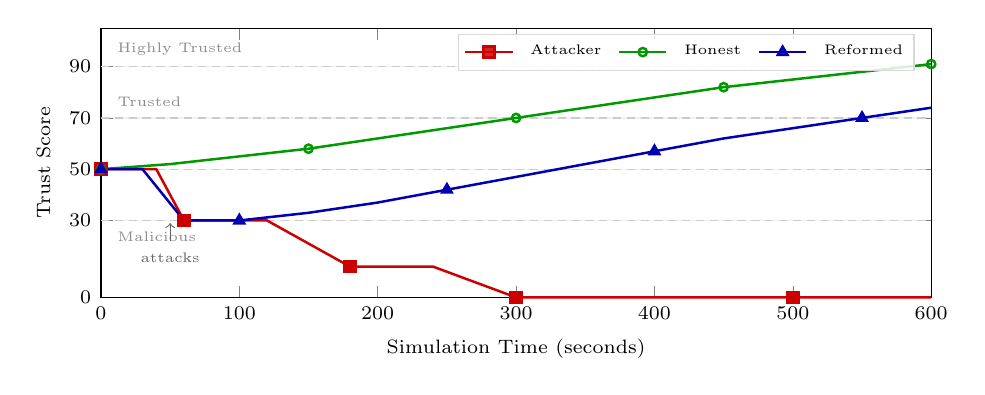
\begin{tikzpicture}
  \begin{axis}[
      width=\columnwidth,
      height=5.0cm,
      xlabel={Simulation Time (seconds)},
      ylabel={Trust Score},
      xmin=0, xmax=600,
      ymin=0, ymax=105,
      ytick={0,30,50,70,90},
      tick label style={font=\scriptsize},
      label style={font=\scriptsize},
      clip=false,
      ymajorgrids=true,
      grid style={gray!12},
      legend style={
          at={(0.98,0.98)},
          anchor=north east,
          font=\tiny,
          draw=gray!30,
          fill=white,
          legend columns=-1,
          column sep=4pt,
          inner sep=2pt,
          fill opacity=0.85,
          text opacity=1,
      },
      every axis plot/.append style={line width=1.2pt},
  ]

  % --- Tier boundary lines ---
  \draw[black!20, densely dashed, thin] (axis cs:0,90) -- (axis cs:600,90);
  \draw[black!20, densely dashed, thin] (axis cs:0,70) -- (axis cs:600,70);
  \draw[black!20, densely dashed, thin] (axis cs:0,50) -- (axis cs:600,50);
  \draw[black!20, densely dashed, thin] (axis cs:0,30) -- (axis cs:600,30);

  % --- Tier labels (inside plot, left side) ---
  \node[font=\tiny, anchor=south west, black!45] at (axis cs:5,90.5) {Highly Trusted};
  \node[font=\tiny, anchor=south west, black!45] at (axis cs:5,70.5) {Trusted};
  \node[font=\tiny, anchor=north west, black!45] at (axis cs:5,29.5) {Malicious};

  % --- Line 1: Persistent attacker (drops to 0) ---
  % 1st attack ~60s: -20 (prefix hijack) -> 30
  % 2nd attack ~180s: -18 (subprefix hijack) -> 12
  % 3rd attack ~300s: -18 base + -30 repeat = clamped to 0
  \addplot[red!80!black, solid, line width=0.9pt, mark=square*, mark size=2pt, mark repeat=2]
      coordinates {
      (0,50) (40,50) (60,30) (120,30) (180,12) (240,12) (300,0) (400,0) (500,0) (600,0)
      };
  \addlegendentry{Attacker}

  % --- Line 2: Always honest (climbs to Trusted tier 70+) ---
  % +1 per 100 legit, +5 monthly eval, +10 highly trusted bonus
  \addplot[green!60!black, solid, line width=0.9pt, mark=o, mark size=1.5pt, mark repeat=3]
      coordinates {
      (0,50) (50,52) (100,55) (150,58) (200,62) (250,66) (300,70)
      (350,74) (400,78) (450,82) (500,85) (550,88) (600,91)
      };
  \addlegendentry{Honest}

  % --- Line 3: Misconfigured then reformed ---
  % 1 attack at ~60s (-20), then clean behavior recovery to Trusted (70+)
  \addplot[blue!70!black, solid, line width=0.9pt, mark=triangle*, mark size=2pt, mark repeat=3]
      coordinates {
      (0,50) (30,50) (60,30) (100,30) (150,33) (200,37)
      (250,42) (300,47) (350,52) (400,57) (450,62) (500,66) (550,70) (600,74)
      };
  \addlegendentry{Reformed}

  % --- Annotation: attack events ---
  \draw[->, thin, black!60] (axis cs:50,22) -- (axis cs:50,29);
  \node[font=\tiny, black!60, anchor=north] at (axis cs:50,21) {attacks};

  \end{axis}
  \end{tikzpicture}
  \caption{Trust score trajectories for three non-RPKI AS behavioral profiles on the representative 200-AS topology. A persistent attacker drops from Neutral (50) to Malicious (0) within a
  few consensus rounds as penalties accumulate ($-20$ base $+ -30$ repeat $+ -50$ persistent). A consistently honest AS climbs gradually through legitimate announcements ($+1$ per 100) and
  monthly evaluations ($+5$). A misconfigured-then-reformed AS drops to Suspicious after a single attack, then recovers to Neutral through sustained clean behavior, demonstrating that
  BGP-Sentry supports rehabilitation rather than permanent exclusion.}
  \label{fig:trust_recovery}
  \end{figure}





The PoP consensus mechanism uses a capped threshold formula $\max(3, \min(\lfloor N/3 \rfloor + 1, 5))$, yielding 5 required signatures for all tested scales. Consensus commit rate shows an expected trade-off with network size: 86.6\% at 100 nodes decreasing to 7.1\% at 1{,}000 nodes, because more nodes compete for the signature threshold within the 30-second timeout. Transactions that do not reach consensus are still committed with ``insufficient consensus'' or ``single witness'' status, ensuring no observations are lost. Capacity-limited buffers with TTL-based eviction (Section~\ref{sec:architecture}) kept per-node memory stable across all scales; no buffer overflow or out-of-memory condition was observed even at 1{,}000 nodes processing 2.51M P2P messages.

The BGPCOIN token economy functioned correctly across all scales. Rewards were distributed proportionally to participation: nodes that committed more blocks and voted more frequently accumulated higher balances. Total BGPCOIN distributed ranged from 8,505 (1{,}000 ASes) to 38,721 (100 ASes). Blockchain integrity was verified through SHA-256 hash chain and Merkle root validation for every block in every run.


\subsection{Scoring Trajectory \& Reputation Dynamics}
%Focus: The Life of an AS: Building trust, the cost of an attack, and recovery trajectory.
 

% =======================
% Post-Hoc Forensic Audit Capability
% Demonstrates blockchain auditability (Contribution #3)
% =======================
\subsection{Post-Hoc Forensic Audit}
\label{subsec:posthoc_audit}

Because every BGP observation is recorded as an immutable blockchain transaction with full metadata, operators can reconstruct the complete behavioral history of any AS at any time. Table~\ref{tab:forensic_audit} presents post-hoc forensic queries across all four datasets: the system correctly identified all 16 attacker ASes (4 per dataset) and their specific attack types from blockchain records alone. Persistent attackers (PREFIX\_HIJACK, SUBPREFIX\_HIJACK, BOGON\_INJECTION) were driven to trust scores of 0 (Malicious), while intermittent attackers (ROUTE\_FLAPPING) remained Suspicious. The blockchain provides a complete, tamper-evident audit trail for retrospective security analysis without access to the original BGP feeds.

\anik{Beyond the basic attacker identification, we evaluate the four post-hoc forensic capabilities described in Section~\ref{subsec:posthoc_building_blocks}. Table~\ref{tab:posthoc_results} summarizes findings across three CAIDA-derived topologies (50, 100, and 200~ASes). At 200~ASes, cross-observer correlation filtered xyz single-observer flapping flags as localized convergence artifacts, all confirmed as false positives against ground truth. Coordinated attack detection identified 23 temporal clusters where multiple distinct attacker ASes launched attacks within a 30 second window; the largest cluster involved 5~ASes information invisible to the per-event reactive pipeline. The number of coordination clusters scales with topology size (4 at 50~ASes, 16 at 100, 23 at 200). Observer integrity auditing flagged 14 observers at 200~ASes with false positive rates exceeding $2\sigma$ above the population mean, all attributable to the route flapping detector. Behavioral pattern detection flagged AS545 at 200~ASes for potential trust score gaming, exhibiting 3+ distinct attack phases separated by clean periods.}

\anik{
\begin{table}[t]
\centering
\caption{Post-Hoc Forensic Analysis Results}
\label{tab:posthoc_results}
\resizebox{\columnwidth}{!}{%
\scriptsize\setlength{\tabcolsep}{4pt}
\begin{tabular}{lrrr}
\toprule
\textbf{Analysis} & \textbf{50 ASes} & \textbf{100 ASes} & \textbf{200 ASes} \\
\midrule
\multicolumn{4}{l}{\textit{(i) Cross-Observer Route Stability}} \\
\quad Prefixes flagged (real-time) & 102 & 209 & 136 \\
\quad Systemic (multi-observer) & 101 & 209 & 109 \\
\quad Localized / FPs filtered & 1 & 0 & 27 \\
\midrule
\multicolumn{4}{l}{\textit{(iii) Coordinated Attack Detection}} \\
\quad Coordination clusters & 4 & 16 & 23 \\
\quad Max attackers per cluster & 2 & 4 & 5 \\
\midrule
\multicolumn{4}{l}{\textit{(iv) Observer Integrity Auditing}} \\
\quad Observers audited & 50 & 100 & 200 \\
\quad Outliers ($>$2$\sigma$ FP rate) & 1 & 2 & 14 \\
\midrule
\multicolumn{4}{l}{\textit{(v) Behavioral Pattern Detection}} \\
\quad ASes with attacks & 3 & 9 & 13 \\
\quad Multi-phase attackers & 0 & 3 & 1 \\
\quad Gaming pattern detected & 0 & 0 & 1 \\
\bottomrule
\end{tabular}}
\end{table}
}
